\documentclass[12pt, a4paper, twoside]{article}

%% Preamble
\usepackage{umatfgenglish}
\usepackage{blindtext}
\usepackage[backend = biber, hyperref,backref = true, style=ieee]{biblatex}
\usepackage{hyperref}
\usepackage{fontspec}
\usepackage{amsmath}

\addbibresource{references.bib}
\graphicspath{{images/}{../images/}}

\setmonofont{[Iosevka.ttf]}

\definecolor{mygreen}{rgb}{0,0.6,0}
\definecolor{mygray}{rgb}{0.5,0.5,0.5}
\definecolor{mymauve}{rgb}{0.58,0,0.82}
\definecolor{codebg}{HTML}{fafafa}

\hypersetup{
  colorlinks,
  linkcolor={red!50!black},
  citecolor={blue!50!black},
  urlcolor={blue!80!black}
}

\lstset{ 
  backgroundcolor=\color{codebg},   % choose the background color; you must add \usepackage{color} or \usepackage{xcolor}; should come as last argument
  basicstyle=\ttfamily,        % the size of the fonts that are used for the code
  breakatwhitespace=false,         % sets if automatic breaks should only happen at whitespace
  breaklines=true,                 % sets automatic line breaking
  captionpos=b
  commentstyle=\color{mygreen},    % comment style
  deletekeywords={...},            % if you want to delete keywords from the given language
  escapeinside={\%*}{*)},          % if you want to add LaTeX within your code
  extendedchars=true,              % lets you use non-ASCII characters; for 8-bits encodings only, does not work with UTF-8
  inputpath=code,
  keepspaces=true,                 % keeps spaces in text, useful for keeping indentation of code (possibly needs columns=flexible)
  keywordstyle=\color{blue},       % keyword style
  language=Scala,                  % the language of the code
  morekeywords={*,\$},             % if you want to add more keywords to the set
  showspaces=false,                % show spaces everywhere adding particular underscores; it overrides 'showstringspaces'
  showstringspaces=false,          % underline spaces within strings only
  showtabs=false,                  % show tabs within strings adding particular underscores
  stepnumber=2,                    % the step between two line-numbers. If it's 1, each line will be numbered
  stringstyle=\color{mymauve},     % string literal style
  tabsize=2,	                     % sets default tabsize to 2 spaces
}

\usepackage{subfiles} % Best loaded last in the preamble

\begin{document}

%% Cover
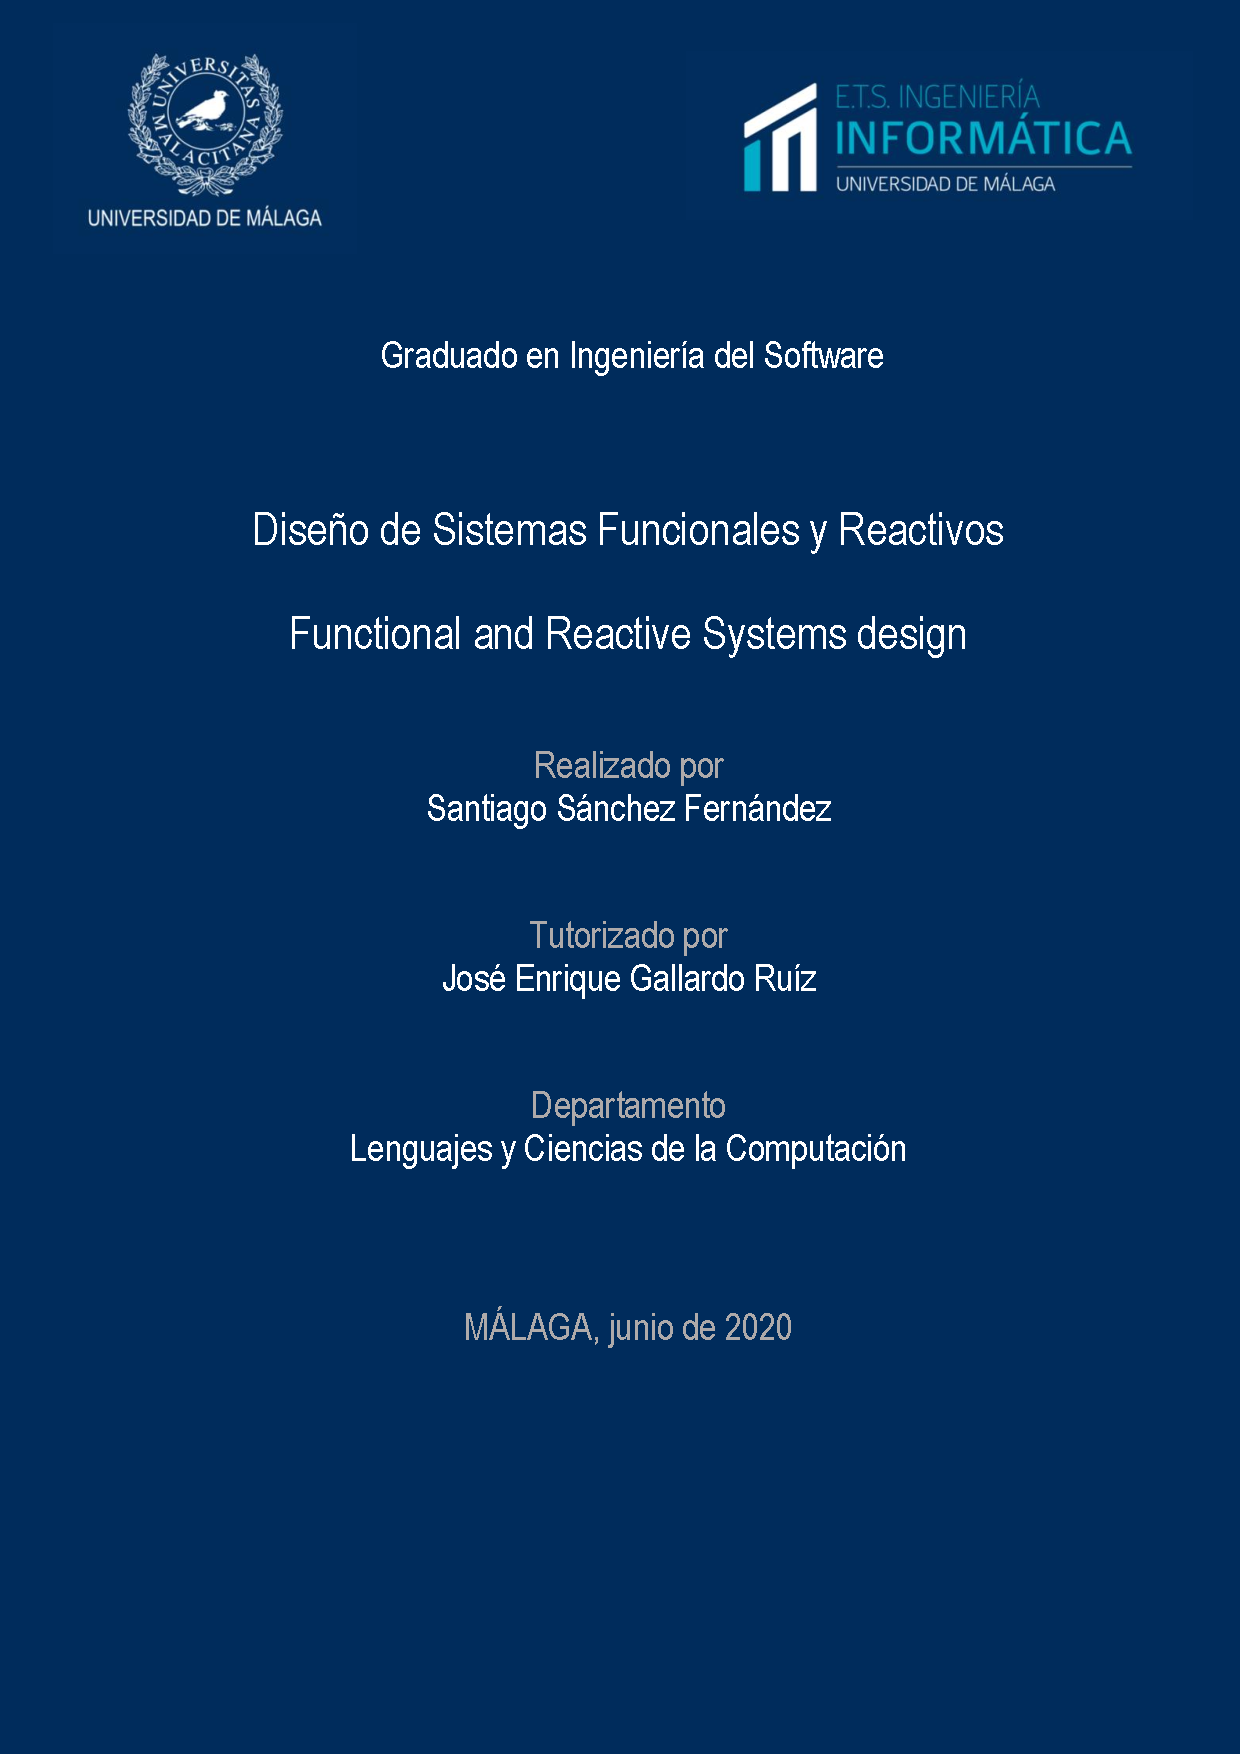
\includepdf[noautoscale=true, width=\paperwidth]{cover.pdf}

%% Title
\clearpage
\setcounter{page}{1}

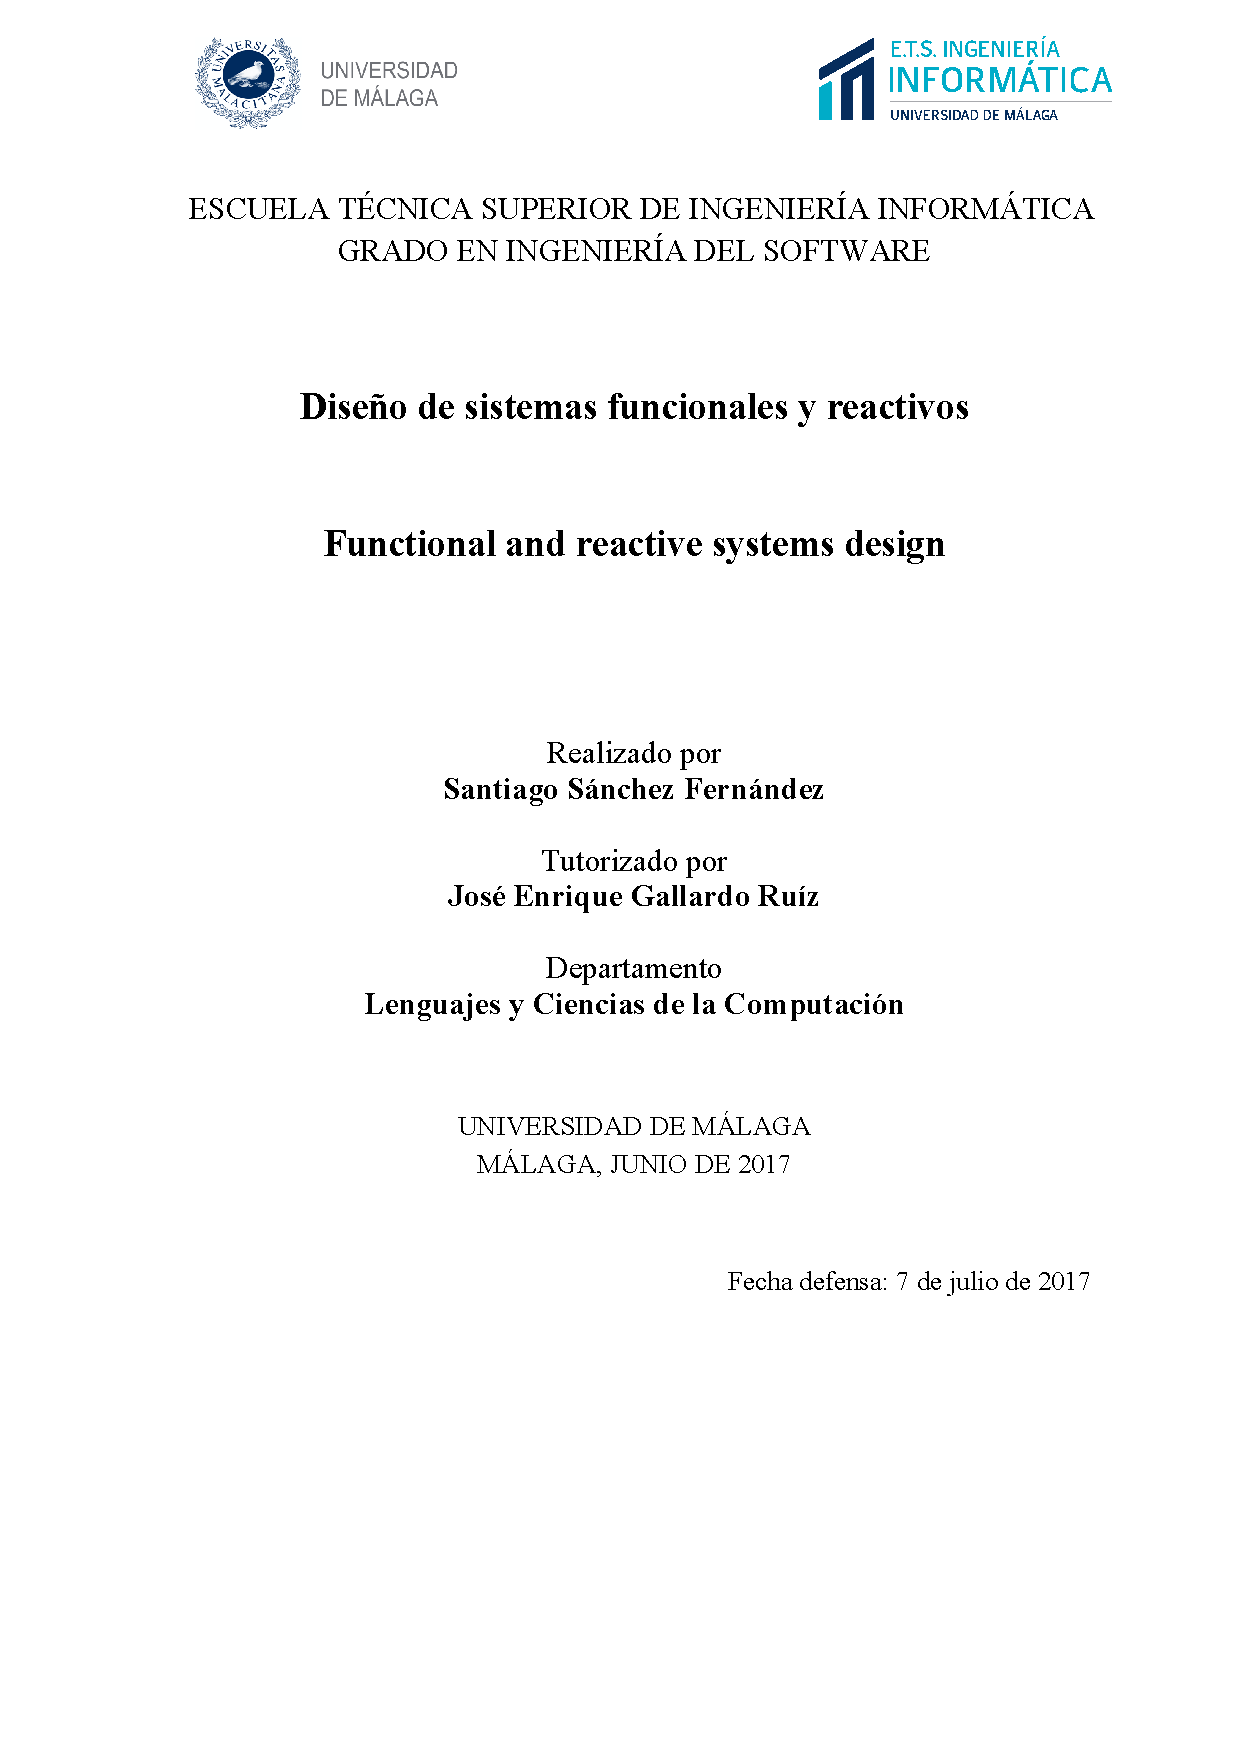
\includepdf[noautoscale=true, width=\paperwidth]{title.pdf}

\newpage

%% Abstract
\subfile{sections/abstract}

\newpage

\subfile{sections/resumen}

\tableofcontents

%% Sections
\section{Introduction}
\subfile{sections/introduction}

\section{Concepts of Functional Programming}
\subfile{sections/functionalprogramming}

\section{Reactive Systems}
\subfile{sections/reactivesystems}

\section{Elements of Functional and Reactive Systems}
\subfile{sections/patterns}

\section{Building a Functional and Reactive Application}
\subfile{sections/programs}

\section{Conclusions and Futures Lines of Research}
\subfile{sections/conclusion}

\section{Conclusiones y Líneas Futuras}
\subfile{sections/conclusiones}

%% Bibliography
\printbibliography

\newpage

%% Apendices
\begin{umaappendices}
  \section{Installation \\ Manual}

  \textbf{\large{Requirements:}} Unix environment with a Bash shell and PostgreSQL database instance with the name \texttt{fairplay} running in port 5432.

  Download the associated source code and navigate to the root folder \texttt{FairPlay}
  There run the following commands in a Bash shell
  
  \texttt{chmod +x sbt}
  
  \texttt{./sbt run}
  
  The web server will be exposed in the port 8080

\end{umaappendices}

%% Back Cover

\includepdf[noautoscale=true, width=\paperwidth]{backcover.pdf}
\end{document}
